\section{Box method - A short introduction}\label{box}

For the spatial discretization the so called BOX-method is used which unites the advantages of the finite-volume (FV) and finite-element (FE) methods. 

First, the model domain $G$ is discretized with a FE mesh consisting of nodes i and corresponding elements $E_k$. Then, a secondary FV mesh is constructed by connecting the midpoints and barycenters of the elements surrounding node i creating a box $B_i$ around node i (see Figure \ref{pc:box}a). 

\begin{figure} [h]
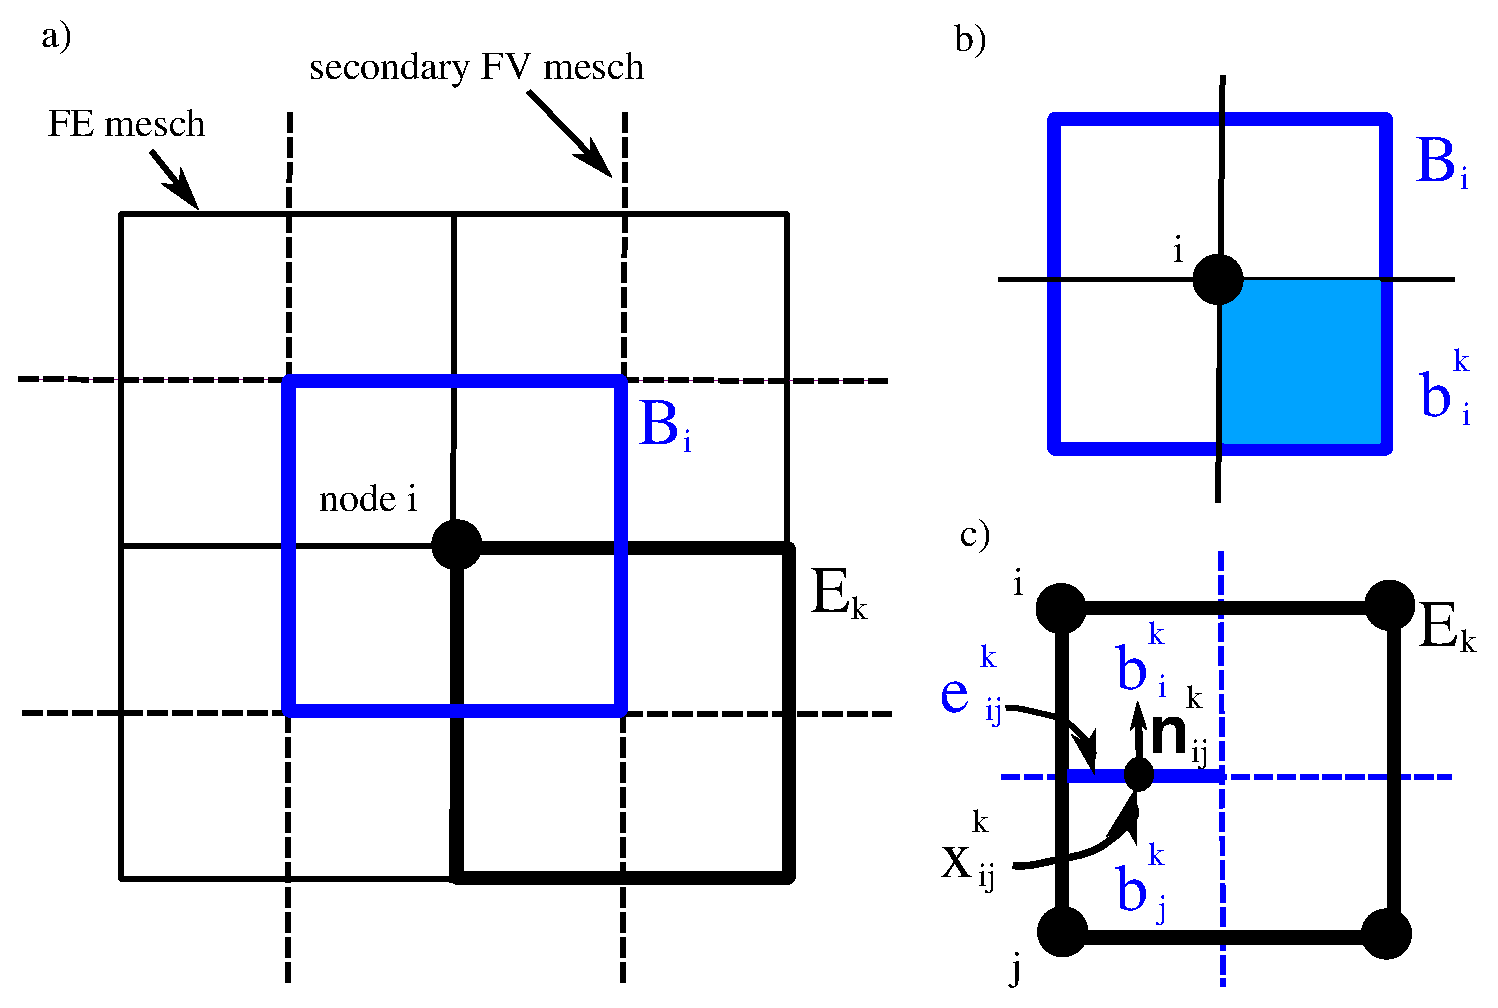
\includegraphics[width=0.8\linewidth,keepaspectratio]{EPS/box_disc}
\caption{\label{pc:box} Discretization of the BOX-method}
\end{figure}

The FE mesh divides the box $B_i$ into subcontrolvolumes (scv's) $b^k_i$ (see Figure \ref{pc:box}b). Figure \ref{pc:box}c shows the finite element $E_k$ and the scv's $b^k_i$ inside $E_k$, which belong to four different boxes $B_i$. Also necessary for the discretization are the faces of the subcontrolvolumes (scvf's) $e^k_{ij}$ between the scv's $b^k_i$ and $b^k_j$, where $|e^k_{ij}|$ is the length of the scvf. The integration points $x^k_{ij}$ on $e^k_{ij}$ and the outer normal vector $\mathbf n^k_{ij}$ are also to be defined (see Figure \ref{pc:box}c).

The advantage of the FE method is that unstructured grids can be used, while the FV method is mass conservative. The idea is to apply the FV method (balance of fluxes across the interfaces) to each FV box $B_i$  and to get the fluxes across the interfaces $e^k_{ij}$ at the integration points $x^k_{ij}$ from the FE approach. Consequently, at each scvf the following expression results:

\begin{equation}
 	f(\tilde u(x^k_{ij})) \cdot \mathbf n^k_{ij} \: |e^k_{ij}| \qquad \textrm{with} \qquad \tilde u(x^k_{ij}) = \sum_i N_i(x^k_{ij}) \cdot \hat u_i .
\end{equation}

In the following, the discretization of the balance equation is going to be derived. From the \textsc{Reynolds} transport theorem follows the general balance equation:

\begin{equation}
	\underbrace{\int_G \frac{\partial}{\partial t} \: u \: dG}_{1} + \underbrace{\int_{\partial G} (\mathbf{v} u + \mathbf w) \cdot \textbf n \: d\varGamma}_{2} = \underbrace{\int_G q \: dG}_{3}
\end{equation}

\begin{equation}
	f(u) = \int_G \frac{\partial u}{\partial t} \: dG + \int_{G} \nabla \cdot \underbrace{\left[  \mathbf{v} u + \mathbf w(u)\right] }_{F(u)}  \: dG - \int_G q \: dG = 0
\end{equation}
where term 1 describes the changes of entity $u$ within a control volume over time, term 2 the advective, diffusive and dispersive fluxes over the interfaces of the control volume and term 3 is the source and sink term. $G$ denotes the model domain and $F(u) = F(\mathbf v, p) = F(\mathbf v(x,t), p(x,t))$.

Like the FE method, the BOX-method follows the principle of weighted residuals. In the function $f(u)$ the unknown $u$ is approximated by discrete values at the nodes of the FE mesh $\hat u_i$ and linear basis functions $N_i$ yielding an approximate function $f(\tilde u)$. For $u\in \lbrace \mathbf v, p, x^\kappa \rbrace$ this means

\begin{minipage}[b]{0.47\textwidth}
\begin{equation}
\label{eq:p} 
	\tilde p = \sum_i N_i \hat{p_i}
\end{equation}
\begin{equation}
\label{eq:v} 
	\tilde{\mathbf v} = \sum_i N_i \hat{\mathbf v}
\end{equation}
\begin{equation}
\label{eq:x} 
	\tilde x^\kappa  = \sum_i N_i \hat x^\kappa 
\end{equation}
\end{minipage}
\hfill
\begin{minipage}[b]{0.47\textwidth}
\begin{equation}
\label{eq:dp} 
	\nabla \tilde p = \sum_i \nabla N_i \hat{p_i}
\end{equation}
\begin{equation}
\label{eq:dv} 
	\nabla \tilde{\mathbf v} = \sum_i \nabla N_i \hat{\mathbf v}
\end{equation}
\begin{equation}
\label{eq:dx} 
	\nabla \tilde x^\kappa  = \sum_i \nabla N_i \hat x^\kappa .
\end{equation}
\end{minipage} 

Due to the approximation with node values and basis functions the differential equations are not exactly fulfilled anymore but a residual $\varepsilon$ is produced.

\begin{equation}
	f(u) = 0  \qquad \Rightarrow \qquad f(\tilde u) = \varepsilon
\end{equation}

Application of the principle of weighted residuals, meaning the multiplication of the residual $\varepsilon$ with a weighting function $W_j$  and claiming that this product has to vanish within the whole domain,

\begin{equation}
	\int_G W_j \cdot \varepsilon \: \overset {!}{=} \: 0 \qquad \textrm{with} \qquad \sum_j W_j =1
\end{equation}
yields the following equation:

\begin{equation}
	\int_G W_j \frac{\partial \tilde u}{\partial t} \: dG + \int_G W_j \cdot \left[ \nabla \cdot F(\tilde u) \right]  \: dG - \int_G W_j \cdot q \: dG = \int_G W_j \cdot \varepsilon \: dG \: \overset {!}{=} \: 0 .
\end{equation}

Then, the chain rule and the \textsc{Green-Gaussian} integral theorem are applied.

\begin{equation}
	\int_G W_j \frac{\partial \sum_i N_i \hat u_i}{\partial t} \: dG + \int_{\partial G}  \left[ W_j \cdot F(\tilde u)\right]  \cdot \mathbf n \: d\varGamma_G + \int_G  \nabla W_j \cdot F(\tilde u)  \: dG - \int_G W_j \cdot q \: dG = 0
\end{equation}

A mass lumping technique is applied by assuming that the storage capacity is reduced to the nodes. This means that the integrals $M_{i,j} = \int_G W_j \: N_i \: dG$ are replaced by the mass lumping term $M^{lump}_{i,j}$ which is defined as:

\begin{equation}
	 M^{lump}_{i,j} =\begin{cases} \int_G W_j \: dG = \int_G N_i \: dG = V_i &i = j\\
	0 &i \neq j\\
	         \end{cases}
\end{equation}
where $V_i$ is the volume of the FV box $B_i$ associated with node i. The application of this assumption in combination with $\int_G W_j \:q \: dG = V_i \: q$ yields

\begin{equation}
	V_i \frac{\partial \hat u_i}{\partial t} + \int_{\partial G}  \left[ W_j \cdot F(\tilde u)\right]  \cdot \mathbf n \: d\varGamma_G + \int_G  \nabla W_j \cdot F(\tilde u)  \: dG- V_i \cdot q = 0 \, .
\end{equation}

Defining the weighting function $W_j$ to be piecewisely constant over a control volume box $B_i$ 

\begin{equation}
	W_j(x) = \begin{cases}
	          1 &x \in B_i \\
		  0 &x \notin B_i\\
	         \end{cases}
\end{equation}

causes $\nabla W_j = 0$:

\begin{equation}
\label{eq:disc1} 
	V_i \frac{\partial \hat u_i}{\partial t} + \int_{\partial B_i}  \left[ W_j \cdot F(\tilde u)\right] \cdot \mathbf n  \;  d{\varGamma}_{B_i} - V_i \cdot q = 0 .
\end{equation}

The consideration of the time discretization and inserting $W_j = 1$ finally lead to the discretized form which will be applied to the mathematical flow and transport equations:

\begin{equation}
\label{eq:discfin} 
	V_i \frac{\hat u_i^{n+1} - \hat u_i^{n}}{\Delta t} + \int_{\partial B_i}  F(\tilde u^{n+1}) \cdot \mathbf n  \;  d{\varGamma}_{B_i} - V_i \: q^{n+1} \: = 0 
\end{equation}
